% Informal talking guide — disjointness work in ADL2Flowchart
% Compile: pdflatex disjointness_report.tex  (twice for TOC)
%          or: latexmk -pdf disjointness_report.tex

\documentclass[11pt,a4paper]{article}

\usepackage[T1]{fontenc}
\usepackage[utf8]{inputenc}
\usepackage{lmodern}
\usepackage{geometry}
\geometry{margin=2.2cm}
\usepackage{hyperref}
\usepackage{enumitem}
\usepackage{listings}
\usepackage{xcolor}
\usepackage{tikz}
\usetikzlibrary{arrows.meta, positioning}

\hypersetup{colorlinks=true, linkcolor=blue!55!black, urlcolor=blue!55!black}

\definecolor{codebg}{RGB}{248,248,248}
\lstset{
  basicstyle=\ttfamily\small,
  backgroundcolor=\color{codebg},
  frame=single,
  breaklines=true
}

\setlist[itemize]{topsep=4pt, itemsep=2pt}
\setlist[enumerate]{topsep=4pt, itemsep=2pt}

\title{\textbf{Talking guide: disjointness \& region analysis}\\[0.3em]
\large What we added to \texttt{smash} and how to demo it}
\author{}
\date{June 2026}

\begin{document}
\maketitle

\noindent\textbf{What this is:} notes for a conversation with collaborators --- not a paper.
Use it as a script: what we built, why it matters, what to try live, and what \emph{not}
to over-claim.

\tableofcontents
\newpage

%-----------------------------------------------------------------------------
\section{The one-sentence pitch}
%-----------------------------------------------------------------------------

We taught \texttt{./smash} to read an ADL file and answer, for each pair of regions:
\emph{can the same event pass both?} or \emph{are they forced apart?} --- using
heuristics plus optional Z3 proofs on the cuts we can extract.

%-----------------------------------------------------------------------------
\section{Why we bothered}
%-----------------------------------------------------------------------------

\begin{itemize}
  \item Signal regions in one card often look related (SR1 vs SR6, etc.).
  \item Before this work, we only had flowcharts --- no static check for overlap/disjointness.
  \item Useful for: combination studies, catching accidental double-counting, sanity-checking
        reinterpretation maps.
\end{itemize}

\textbf{Scope we're honest about:} single file only, and only the cuts the extractor
understands. If half the cuts are weird BDTs, the tool will say so (coverage warnings).

%-----------------------------------------------------------------------------
\section{What changed --- quick timeline}
%-----------------------------------------------------------------------------

Talk through this in order if people want the story:

\begin{enumerate}
  \item \textbf{Make real ADL parse.} Example corpus went 49/68 $\rightarrow$ 68/68;
        fixed crashes on Delphes-style files.
  \item \textbf{Object disjointness (\texttt{-r}).} ``Are \texttt{bjets} and \texttt{electrons}
        the same kind of thing?''
  \item \textbf{Region heuristics.} Interval clashes on \texttt{MET.pT}, \texttt{size(bjets)}, tags.
  \item \textbf{Constraint IR + JSON.} Structured per-region facts for tooling.
  \item \textbf{Z3 (SMT).} SAT = overlap proved (with witness); UNSAT = disjoint proved.
  \item \textbf{Robustness pass.} Index-safe keys (\texttt{jets[0]} vs \texttt{jets[1]}),
        \texttt{size} as Int, \texttt{dPhi} in SMT.
  \item \textbf{OR / ITE.} \texttt{A || B} and \texttt{size >= 3 ? dPhi(...) : ALL} like Delphes presel.
\end{enumerate}

%-----------------------------------------------------------------------------
\section{How to run it (demo script)}
%-----------------------------------------------------------------------------

\begin{lstlisting}
make
./smash -r myfile.adl                    # analysis + Z3 if installed
./smash -r --no-smt myfile.adl           # fast, heuristics only
./smash -r --json out.json myfile.adl    # machine-readable
make test-disjoint                       # small golden tests
\end{lstlisting}

\textbf{Good demo files:}
\begin{itemize}
  \item \texttt{tests/golden/disjoint\_pt.adl} --- clear PROVEN DISJOINT
  \item \texttt{tests/golden/size\_bjets.adl} --- PROVEN OVERLAPPING (subset of multiplicity cuts)
  \item \texttt{examples/CMS/CMS-SUS-16-033\_Delphes.adl} --- real card, many SR pairs
\end{itemize}

%-----------------------------------------------------------------------------
\section{What the output means}
%-----------------------------------------------------------------------------

\begin{description}[style=nextline, leftmargin=2.8cm]
  \item[PROVEN DISJOINT] Intervals clash, or Z3 says UNSAT on $R_1 \wedge R_2$.
        Trust disjoint more than overlap --- UNSAT is sound for what we encoded.
  \item[PROVEN OVERLAPPING] Z3 SAT + regions share a constraint dimension + witness printed.
        Means: \emph{there exists} numbers satisfying both cut sets in our fragment.
        Not the same as ``these SRs have yield in MC.''
  \item[POSSIBLY OVERLAPPING] Heuristic only, or SAT on unrelated knobs (MET vs jet count).
  \item[UNKNOWN] Extraction gap, timeout, or logic we don't encode yet.
\end{description}

%-----------------------------------------------------------------------------
\section{Pipeline sketch (whiteboard version)}
%-----------------------------------------------------------------------------

\begin{center}
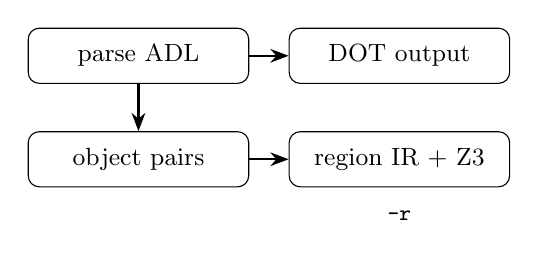
\begin{tikzpicture}[
  box/.style={draw, rounded corners, minimum width=2.8cm, minimum height=0.7cm,
              align=center, font=\small},
  arr/.style={-{Stealth}, thick}
]
  \node[box] (p) {parse ADL};
  \node[box, right=0.5cm of p] (d) {DOT output};
  \node[box, below=0.6cm of p] (o) {object pairs};
  \node[box, right=0.5cm of o] (r) {region IR + Z3};
  \draw[arr] (p) -- (d);
  \draw[arr] (p) -- (o);
  \draw[arr] (o) -- (r);
  \node[font=\footnotesize, below=0.15cm of r] {\texttt{-r}};
\end{tikzpicture}
\end{center}

Main code: \texttt{semantic\_checks.cpp} (extract cuts), \texttt{region\_analysis.cpp} (pairs + Z3).

%-----------------------------------------------------------------------------
\section{What we actually extract}
%-----------------------------------------------------------------------------

\textbf{Works well:}
\begin{itemize}
  \item Scalar cuts: \texttt{MET.pT > 200}, \texttt{pT(jets[0]) > 100}
  \item Multiplicity: \texttt{size(bjets) >= 2}
  \item Tags: \texttt{BTag == 1}
  \item Angular: \texttt{dPhi(jets[0], MHT) > 0.5}
  \item Inheritance: \texttt{select presel}
  \item \texttt{reject} (complemented)
  \item OR and Delphes-style ITE (v3)
\end{itemize}

\textbf{Still weak / skipped:}
\begin{itemize}
  \item BDT scores, arbitrary functions
  \item Deeply nested OR/ITE
  \item Cross-file name alignment
\end{itemize}

Watch the line \texttt{N/M SMT-encodable} and coverage warnings --- if it's low, don't
treat Z3 verdicts as the full story.

%-----------------------------------------------------------------------------
\section{Gotchas worth mentioning}
%-----------------------------------------------------------------------------

\begin{itemize}
  \item \textbf{Different jet indices are not disjoint.} \texttt{jets[0].pt > 300} and
        \texttt{jets[1].pt < 200} can both be true on one event. We fixed a bug where
        those were wrongly merged.
  \item \textbf{Subset $\neq$ disjoint.} \texttt{size >= 4} and \texttt{size >= 2} overlap
        heavily --- Z3 correctly says PROVEN OVERLAPPING.
  \item \textbf{Z3 optional but recommended.} \texttt{apt install z3}; CI expects it.
  \item \textbf{Legacy verbose report} still exists: \texttt{--legacy-region-report} if someone
        wants the old wall of text.
\end{itemize}

%-----------------------------------------------------------------------------
\section{Validation (if someone asks ``is it tested?'')}
%-----------------------------------------------------------------------------

\begin{itemize}
  \item 68/68 files under \texttt{examples/} parse and survive \texttt{-r}
  \item 7 golden ADL fixtures in \texttt{tests/golden/}
  \item GitHub Actions: build + golden + corpus + Delphes Z3 spike
\end{itemize}

%-----------------------------------------------------------------------------
\section{What's next (only if the conversation goes there)}
%-----------------------------------------------------------------------------

\begin{itemize}
  \item Cross-file region comparison
  \item Richer SMT (nested logic, per-jet variables)
  \item Tie witnesses to actual CutLang execution / yields
  \item Clean up Bison grammar conflicts (separate chore)
\end{itemize}

%-----------------------------------------------------------------------------
\section{Suggested 10-minute walkthrough}
%-----------------------------------------------------------------------------

\begin{enumerate}
  \item Show \texttt{./smash -r tests/golden/disjoint\_pt.adl} --- one PROVEN DISJOINT line.
  \item Show \texttt{size\_bjets.adl} --- PROVEN OVERLAPPING + witness.
  \item Open \texttt{CMS-SUS-16-033\_Delphes.adl} --- ``this is a real card, not a toy.''
  \item Show JSON: \texttt{--json /tmp/x.json} and point at \texttt{fragment\_coverage}.
  \item Close with limits: fragment, not full simulation.
\end{enumerate}

\vfill
\noindent\hrulefill

\noindent\small More detail in repo: \texttt{REGION\_ANALYSIS.md},
\texttt{VERIFICATION\_REPORT.md}, \texttt{docs/SMT\_ROBUSTNESS\_PLAN.md}.

\end{document}